\documentclass[../main.tex]{subfiles}
 
\begin{document}

\section{Eszköz (elektronikai és beágyazott szoftverének) tervezése és összeállítása}
    \subsection{Elektronikai tervezés}
        Az elektronikai tervezést 3 fázisra és az utolsó fázis hibáinak kijavítására bontanám le. Az első fázis első lépései között szerepelt az Ebay-ről vásárolt eszközök tesztelése: működik-e mindegyik, programozható-e a fejlesztői lap, konfigurálható-e a Wifi modul, stb\ldots
        
        Második lépésként megnéztem a mikrovezérlőm lábkiosztását (Ábra \ref{fig:stm32f103_pinout}) és az alapján kiválasztottam melyeket fogom használni. 
        
        % https://os.mbed.com/users/hudakz/code/STM32F103C8T6_Hello/wiki/Homepage
        \begin{figure}[h!]
            \centering
                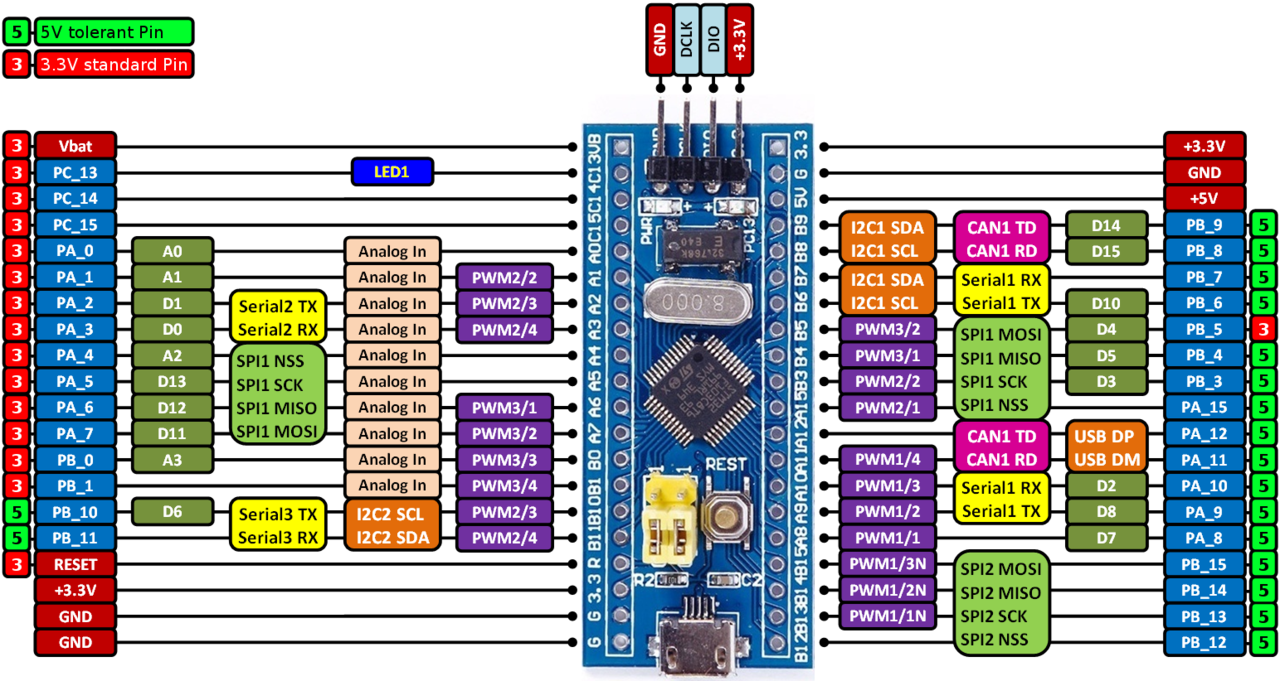
\includegraphics[width=14cm]{resources/pcb_res/stm32f103c8t6_pinout.png}
            \caption{STM32F103C8T6 fejlesztői lap pinout-ja}
            \label{fig:stm32f103_pinout}
        \end{figure}
        
        A PB\_0-s lábat választottam a LED sor vezérlő lábnak, és a PA\_9, PA\_10 (TX,RX) lábakat pedig Wifi modullal kommunikáló UART lábaknak. Minden modulra a megfelelő tápfeszültséget kötöttem, illetve az összes földpotenciált összehuzalosztam, ezátal egy közös földpontot létrehozva. A ESP-01-s modul pinoutja (Ábra \ref{fig:eps01_pinout}) alapján UART lábkat is összekötöttem a megfelelő módon: a mikrovezérlő RX lábát (PA\_10) a Wifi modul U0TXD lábával és mikrovezérlő TX lábát (PA\_9) a Wifi modul U0RXD lábával. 
        
        \begin{figure}[h!]
            \centering
                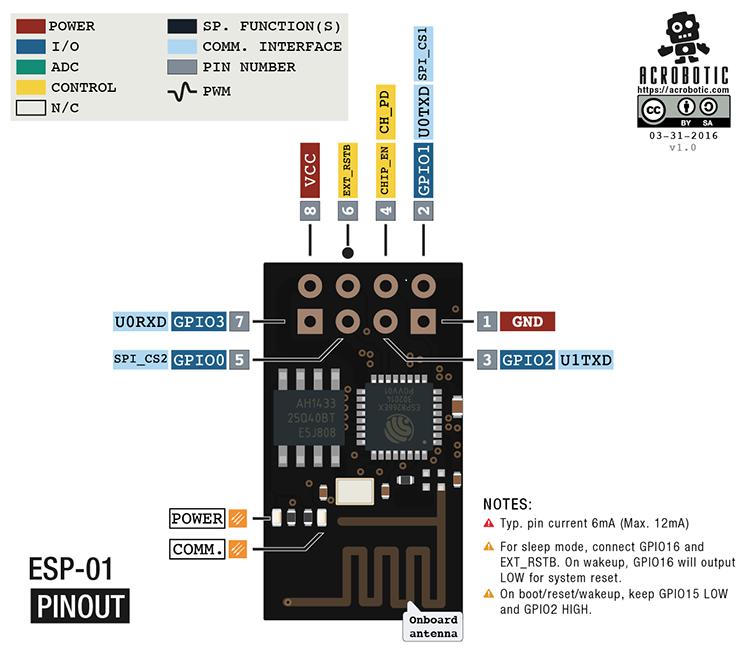
\includegraphics[width=10cm]{resources/pcb_res/esp8266_esp01_pinout.png}
            \caption{ESP-01 pinout-ja}
            \label{fig:eps01_pinout}
        \end{figure}
        
        A WS2811-es IC adatlapján a logikai jelszintes részt áttanulmányozva megállapítottam, hogy a mikrovezérlő 3,3V-os vezérlő jelét még éppen tolerálja a LED sor vezérlő IC 5V-os bemeneti lába (3,2V-os jel igaznak felel meg). 
        
        Ezek alapján összeállítottam a kapcsolást breadboard-on, és az internetről letöltött mintaprogramokat kicsit módosítva elértem, hogy külön-külön működött a Wifi modullal lévő kommunikáció, illetve a LED soron meg tudtam jeleníteni egy fehér színt. Az összeállítással több problémai is volt: a tesztelés során a breadboardból gyakran kicsúsztak a kábelek, a csatlakozások kontaktosak voltak, hamis színeket okozva ezzel a LED soron. 
        
        A problémák orvoslásaként került sor a második fázis kivitelezésére. A Mikrovezérlők c. tantárgy keretében megtanultunk az Autodesk Eagle nevű nyáktervező program használatát. Az internetről letöltöttem és beimportáltam az STM32F103C8T6 mikrovezérlő fejlesztői lapjának
        % https://os.mbed.com/users/hudakz/code/STM32F103C8T6_Hello/wiki/Homepage
        , az ESP8266-os modul ESP-01-es 
        % forras esp libraryra
        típusának a könyvtárait. Létrehoztam egy saját könyvtárt is az Ebay-ről rendelt DC/DC modulnak. Ez a feszültségátalakító állítja elő a 12V-os tápfeszültségből a 3,3V-osat. Egy pár csatlakozó, állatpotjelző LED és ellenállás hozzáadása után összehuzaloztam a megfelelő elemeket. 
        
        \begin{figure}[h!]
            \centering
                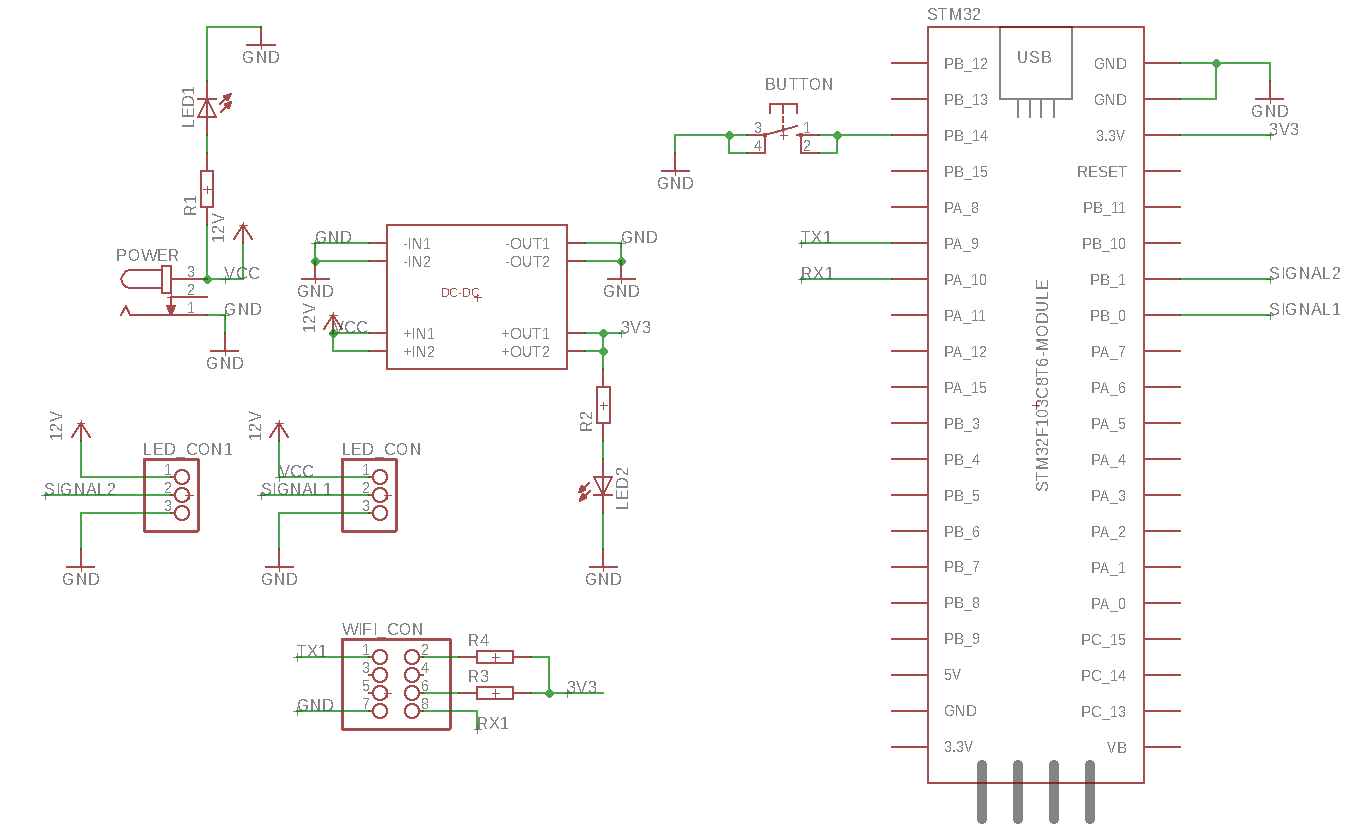
\includegraphics[width=15cm]{resources/pcb_res/schematic_v01.png}
            \caption{2. fázisú kapcsolási rajz}
            \label{fig:schematic_v01}
        \end{figure}
        
        Az elkészült kapcsolási rajz (Ábra \ref{fig:schematic_v01}) után elhelyeztem és összekötöttem az az alkatrészeket az NYÁK-on. Ezen a verzión bekötésre került egy extra gomb (BUTTON) és egy extra csatlakozó (LED\_CON1), hogy mostmár 2 LED sort legyen képes vezérleni az eszköz párhuzamosan. \ref{fig:board_v01}. Ábra szemléltei az így összehuzalozott NYÁK-ot.
        
        \begin{figure}[h!]
            \centering
                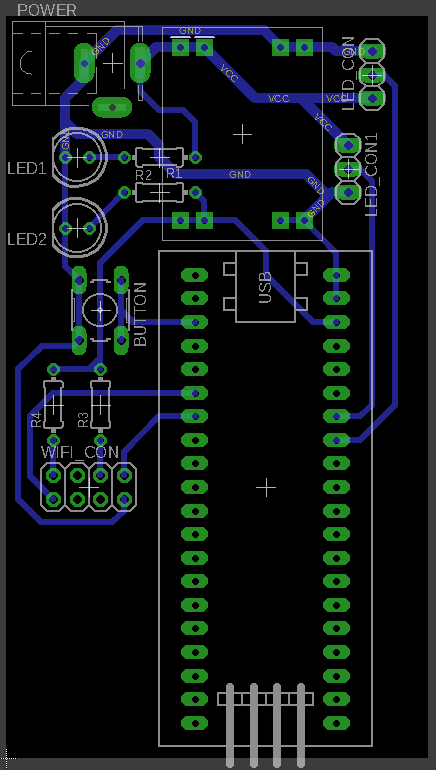
\includegraphics[width=6cm, angle =-90]{resources/pcb_res/board_v01.png}
            \caption{2. fázisú NYÁK-terv}
            \label{fig:board_v01}
        \end{figure}
        
        A NYÁK-ot vasalásos technikával elkészítettem: a tervet fényes papírra lézernyomtatóval kinyomtattam, egy egyoldalas NYÁK-lapra ráhelyeztem, a tonerport vasalóval átvittem a réz felületre, a tonerral nem fedett réz részeket pedig a maratószer lemarattam, és végül acetonnal eltávolítottam, hogy a megmaradt rézfelületre lehessen forrasztani. Az így elkészült NYÁK-ot (Ábra \ref{fig:pcb_v01}) beforrasztottam és az alkatrészeket belehelyeztem. Ezzel a NYÁK-al már el lehetett kezdeni a beágyazott szoftver fejlesztését, az elektronikai rész stabilan működött.
        
        \begin{figure}[h!]
            \centering
                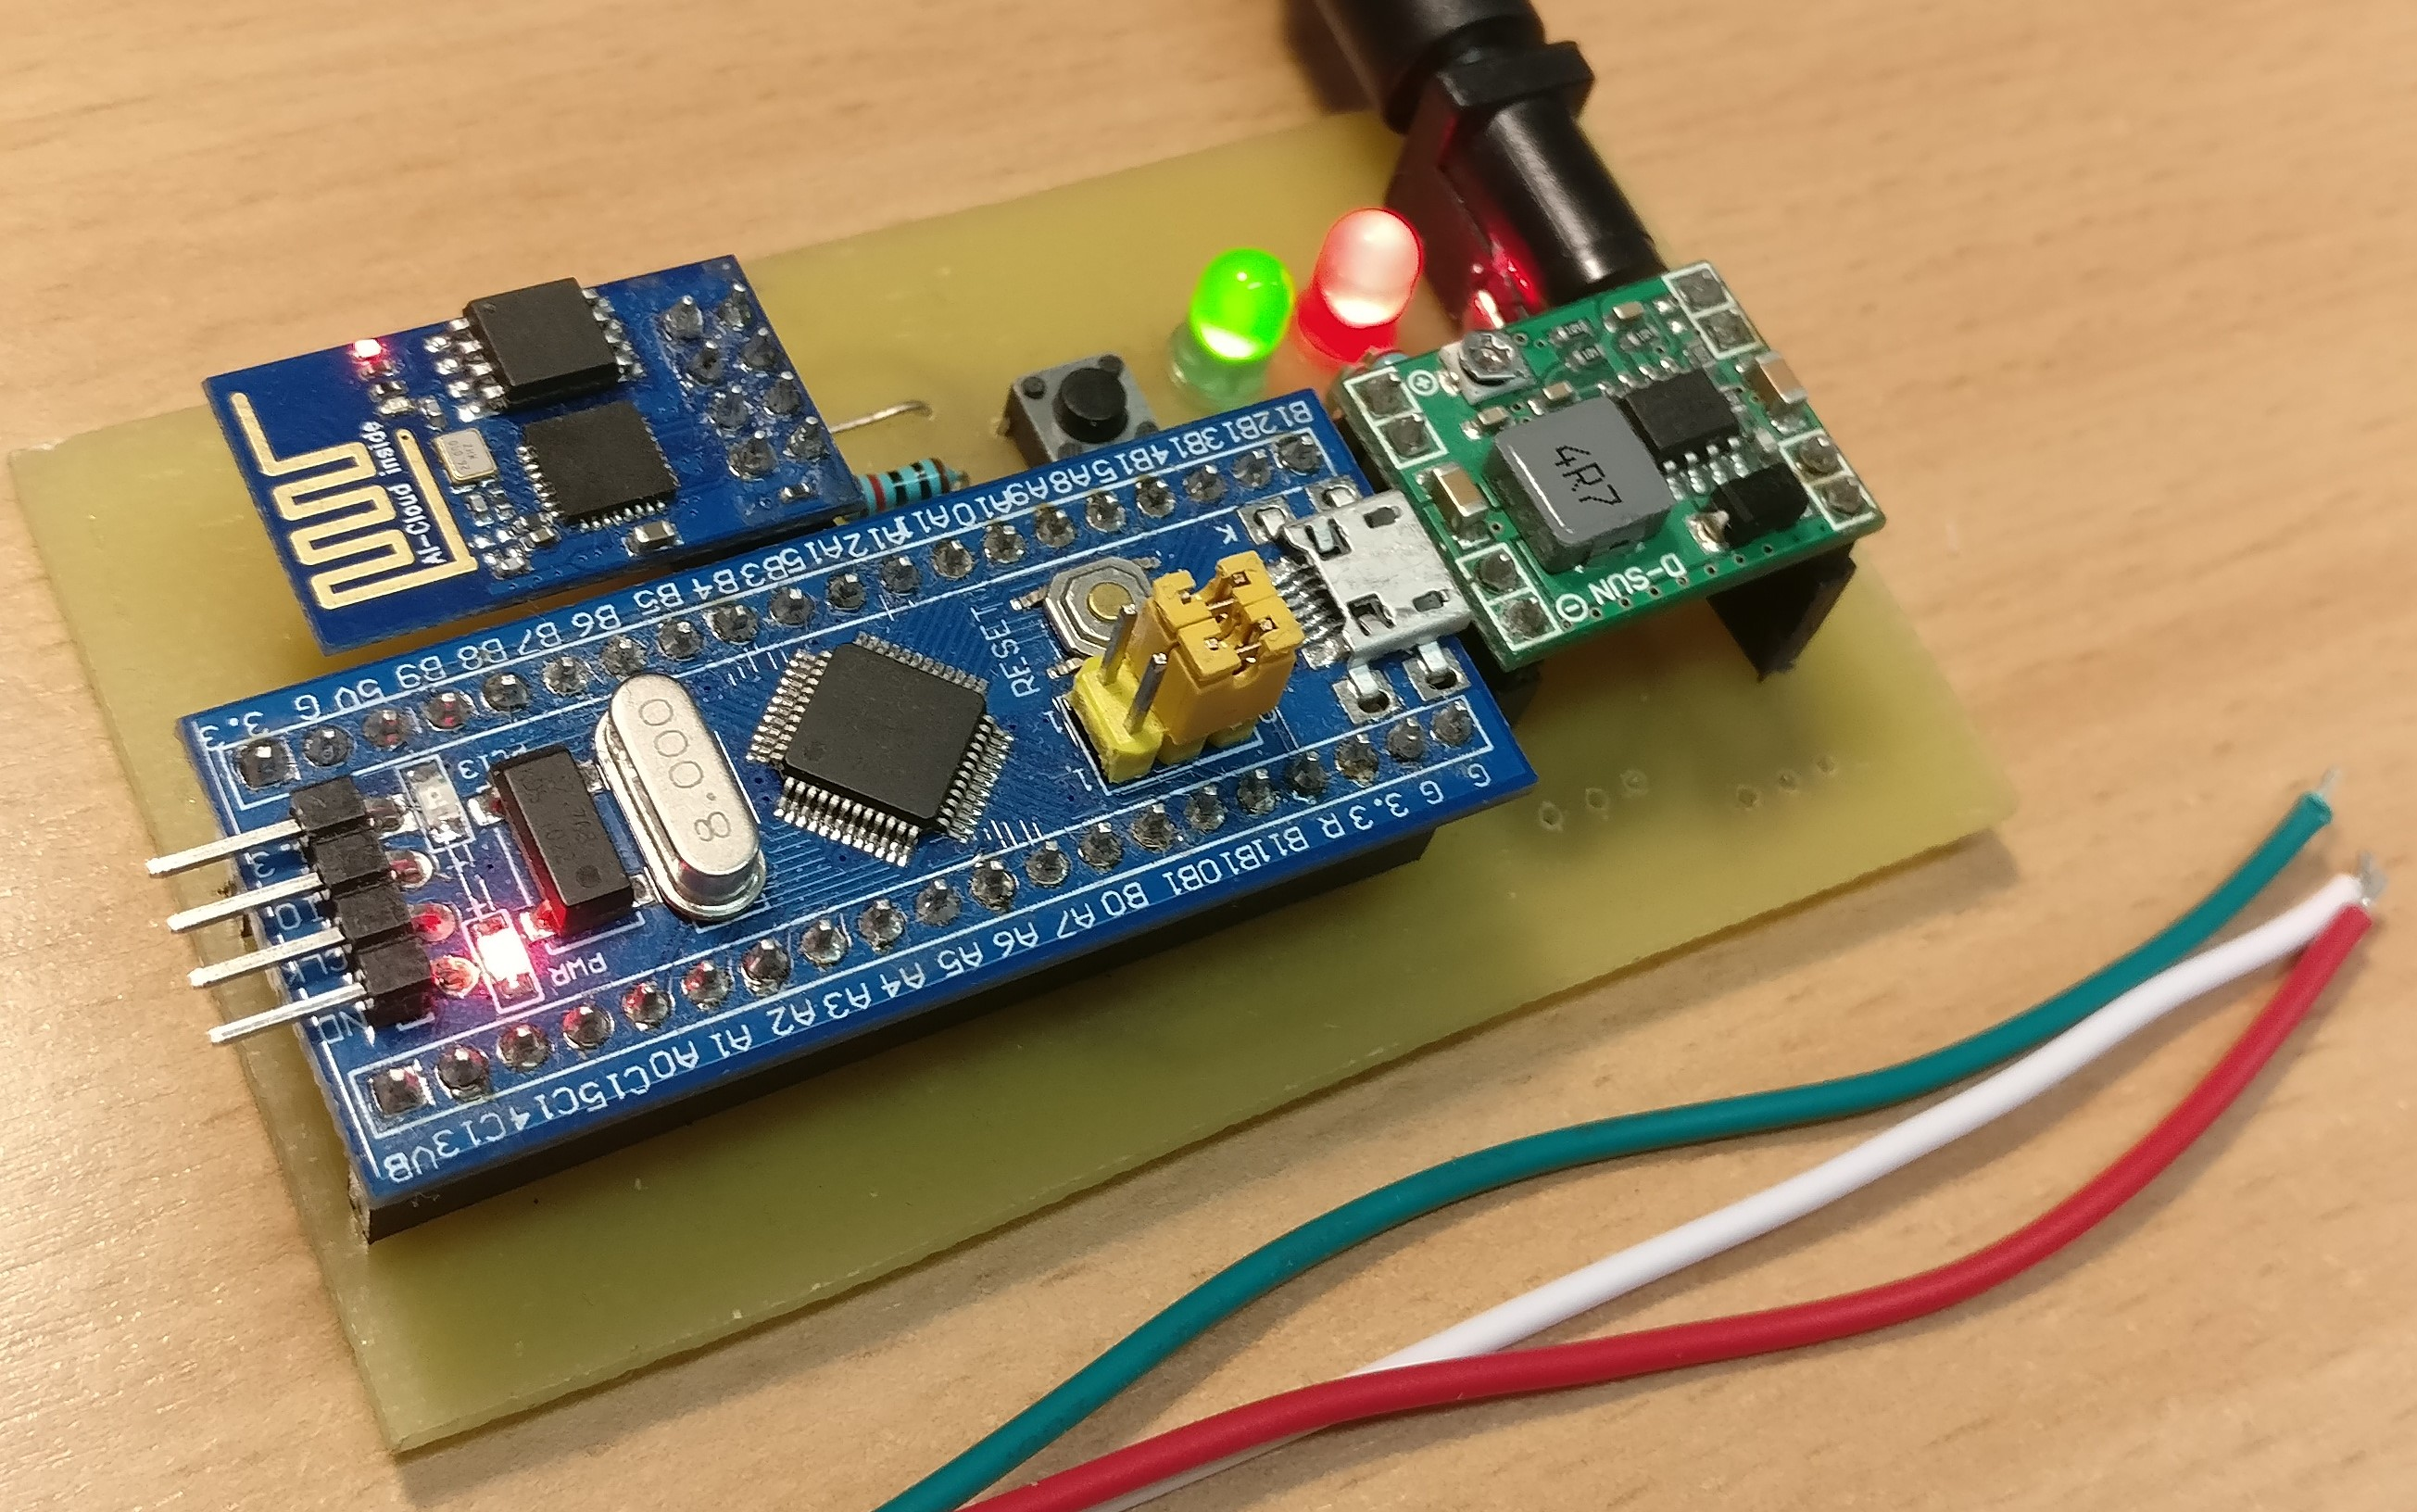
\includegraphics[width=6cm]{resources/pcb_res/pcb_v01.png}
            \caption{2. fázisú beforrasztott áramkör //TODO képet megcsinálni}
            \label{fig:pcb_v01}
        \end{figure}
        
        A 3. fázis tartalmazza DC/DC áramkörök tervezését és mikrovezérlő perifériáival együtti integrálását egy nyomtatott áramköri lapra.
        
        \subsubsection{DC/DC tervezés}
            %https://www.quora.com/Where-can-I-use-LDO-and-DC-DC-converters
            Az én esetemben nagy volt a különbség a bementi és a kimenteti feszültségek között (12V-ról 5V-ra), ezért egy DC/DC konverter sokkal jobban megfelel az én alkalmazásomban mint egy LDO (Low-DropOut regulator), hiszen egy LDO-nak a hatékonysága nagyon alacsony (12V-ról 5V-ra kb. 41\%) és a maradék energiát elfűti. Ez a megoldás semmiképpen sem előnyös, illetve még hűtőborda alkalmazását is megköveteli.
            
            %https://electronics.stackexchange.com/questions/160218/how-does-dcdc-save-power-over-an-ldo
            % zajos 
            % nehezebb a tervezes
            % több komponensből áll
            
            A 3,3V és 5V-os tápfeszültségek ellőállítására 2 DC/DC áramkörre is szükségem volt, és ezért olyan megoldást kerestem, ahol ugyon azzal az IC-vel, külső komponenseinek változtatásával ez megoldható. Továbbá szerettem volna hogyha egy 3 cellás LiPo akkumlátorról is működne az áramkör, ezzel hordozhatóvá téve. A bemeneti feszültségem, 3V-os minimum és 4,2V-os maximum cella feszültségnél, egy 3 cellás LiPo-nál, 9V és 12,6V közzé fog esni. A felső értéket egészre kerekítve és eggyel nagyobbra választva (14V) egy kisebb biztonsági sávot is kaptam.
            A DC/DC áramkörök tervezésénél nagy segítségemre volt a TI (Texas Instruments) Webench Power Designer.
            % https://webench.ti.com/webench5/power/
            A tervezési paramétereket megadva, nem csak egy megfelelő IC-t, hanem egy komplett kapcsolásokat is kínál. A kimenteti névleges áramot, a 3,3V-os kimenteti feszültség esetében, 1,5A-ra választottam (Ábra \ref{fig:ti_we_des_param_3v3}), hogy akár még más áramköri lapkát is képes legyen meghajtani az eszközöm. Az 5V-os kimenet esetén (Ábra \ref{fig:ti_we_des_param_5v}) is túlméreteztem a névleges áramot (0.5A).
            % esp8266 datasheet
            % https://www.espressif.com/sites/default/files/documentation/0a-esp8266ex_datasheet_en.pdf 
            \begin{figure}[h!] % https://webench.ti.com/webench5/power/
                \begin{floatrow}
                    \ffigbox{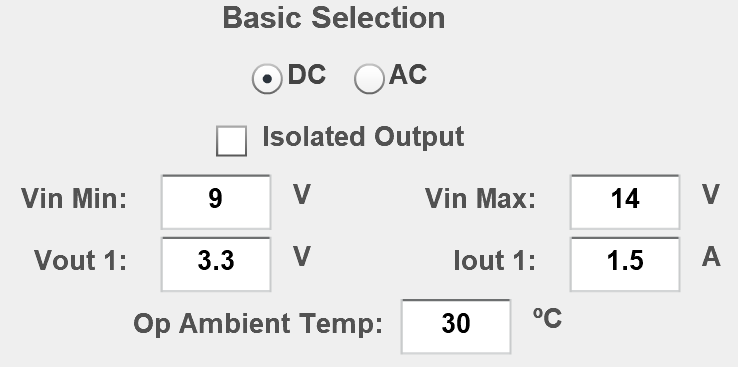
\includegraphics[width=7cm]{resources/pcb_res/ti_we_des_param_3v3.png}}{\caption{Tervezési paraméterek megadása 3,3V-os kimentre}\label{fig:ti_we_des_param_3v3}}
                    \ffigbox{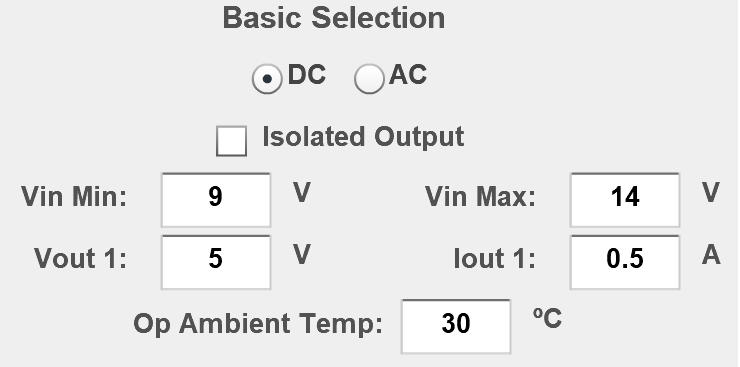
\includegraphics[width=7cm]{resources/pcb_res/ti_we_des_param_5v.png}}{\caption{Tervezési paraméterek megadása 5V-os kimentre}\label{fig:ti_we_des_param_5v}}
                \end{floatrow}
            \end{figure}
            
            Ezek után az integrált, könnyen használható és költséghatékony módszert választva (Ábra \ref{fig:ti_we_des_int_etu_ce_method}) elkezdtem keresgélni a legenerált esetek között, minél olcsóbb és hatékonyabb megoldást keresve.
            
            \begin{figure}[h!]
                \centering
                    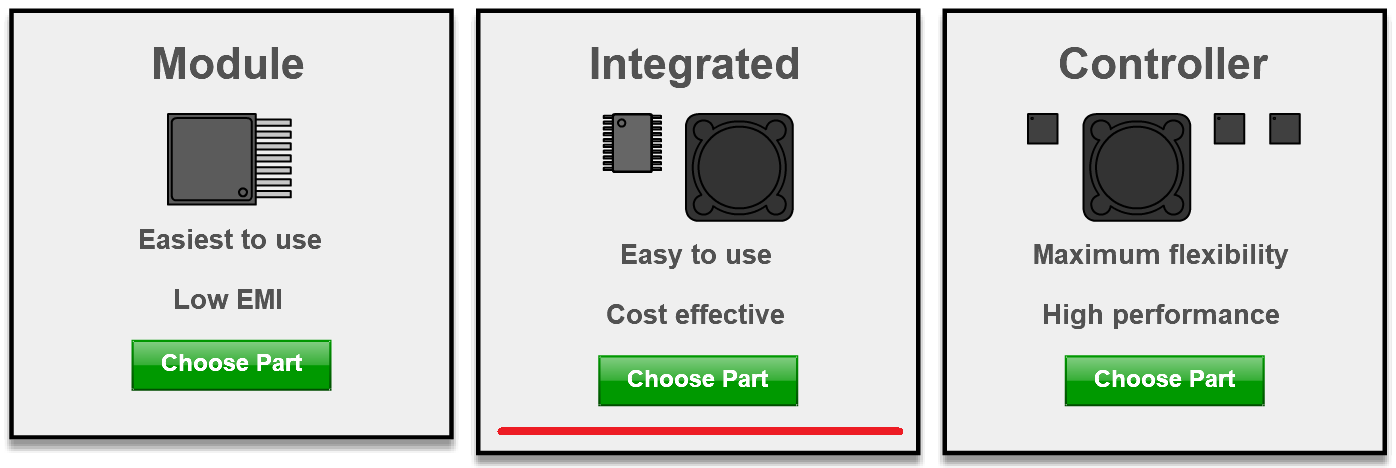
\includegraphics[width=10cm]{resources/pcb_res/ti_we_des_int_etu_ce_method_2.png}
                \caption{Tervezési séma kiválasztása}
                \label{fig:ti_we_des_int_etu_ce_method}
            \end{figure}
            
            A TPS562219A típusú IC mindkét esetben előfordult. A két verzió között (3,3V - 5V) csak egy tekercs és egy ellenállás volt a különbség.
            
            A TI Webench Designer által kínált kapcsolási rajzok, kiválasztott komponensei nem mindig megfelelőek, illetve beszerezhetőek. Tovább bonyolította helyzetet, hogy SMD komponenseket sohasem forrasztottam, tehát az alkatrészek mérete sem volt mindegy számomra. A korábbi tapasztalataim alapján úgy döntöttem hogy 1206-os (metrikus: 3216) SMD méretet fogok használni. Az egyik legnagyobb elektronikai kereskedőnél, a Mouser Electronics-nál, a megfelelő paraméterek figyelembevételével újraválasztottam az alkatrészeket. Miután néhány komponensnek megcsináltam az Eagle könyvtárát, elkészítettem a kapcsolási rajzokat, a Webench Designer és a TPS562219A IC adatlapja alapján. Mivel a két változat (3,3V - 5V) minimálisan különbözik egymástól ezért csak az egyiket ábrázoltam (Ábra \ref{fig:schematic_3v3}).
            
            \begin{figure}[h!]
                \centering
                    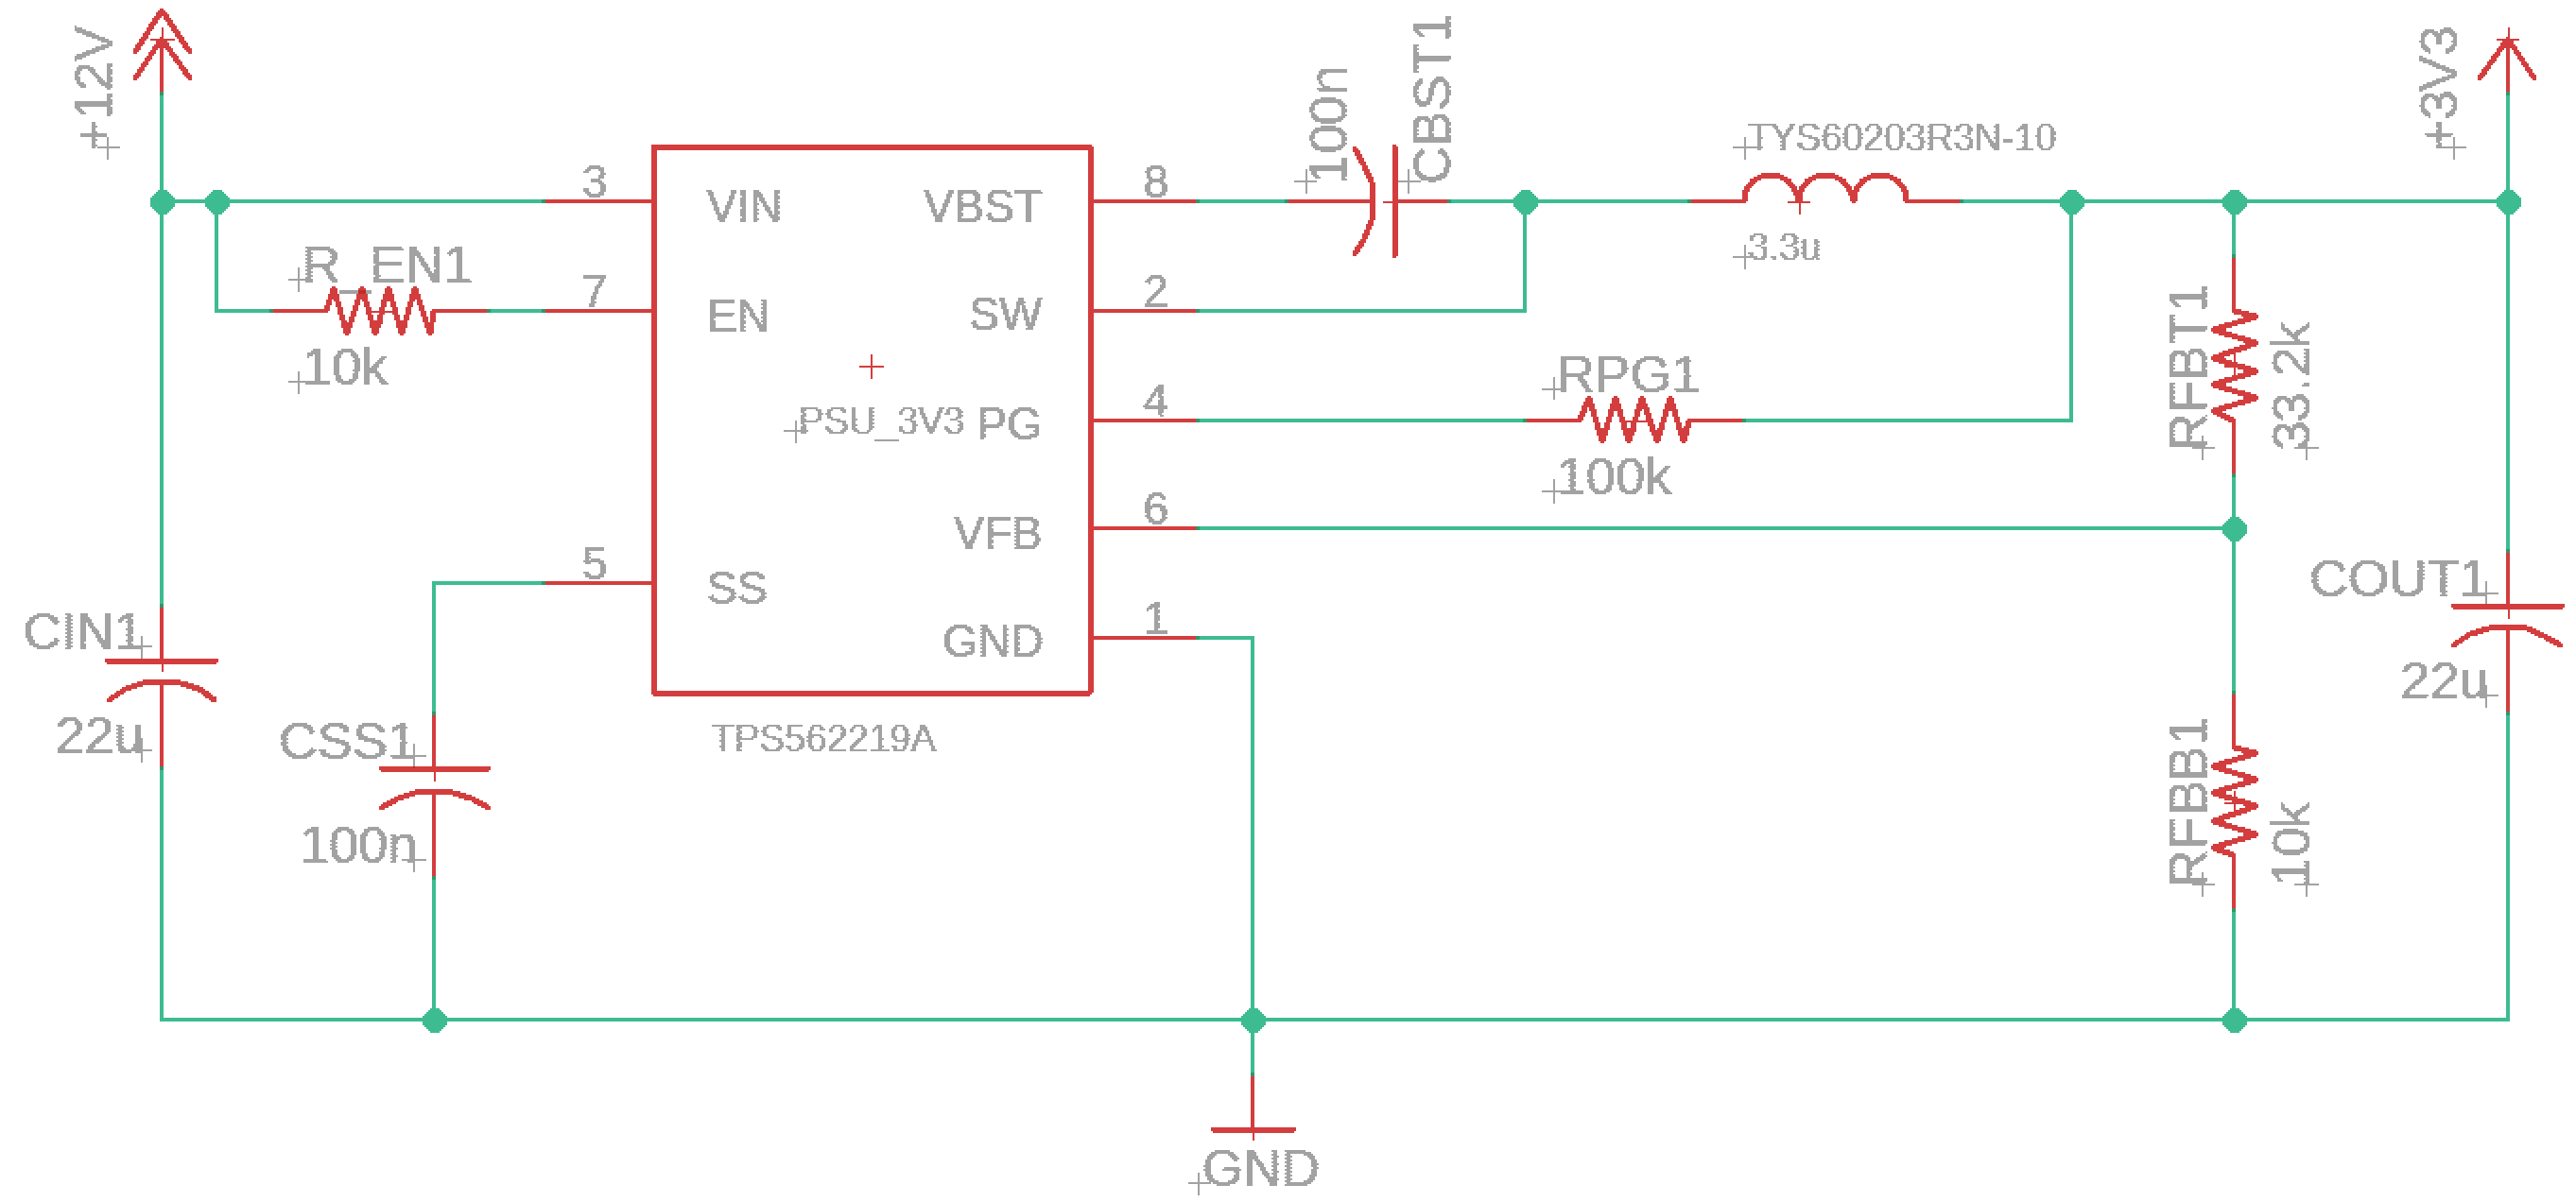
\includegraphics[width=12cm]{resources/pcb_res/schematic_3v3.png}
                \caption{3,3V-os DC/DC kapcsolási rajza}
                \label{fig:schematic_3v3}
            \end{figure}
            
            Általáben nem mindegy, hogy az alkatrészeinket az adott IC körül hogyan helyezzük el. A TPS562219A típusú IC-nek az adatlapjában is pontokba van szedve mire kell odafigyelni, illetve egy elhelyezési mintát (Ábra \ref{fig:tps_logl_example}) is találunk mellete.
            % irányelvek resz
            
            \begin{figure}[h!]
                \centering
                    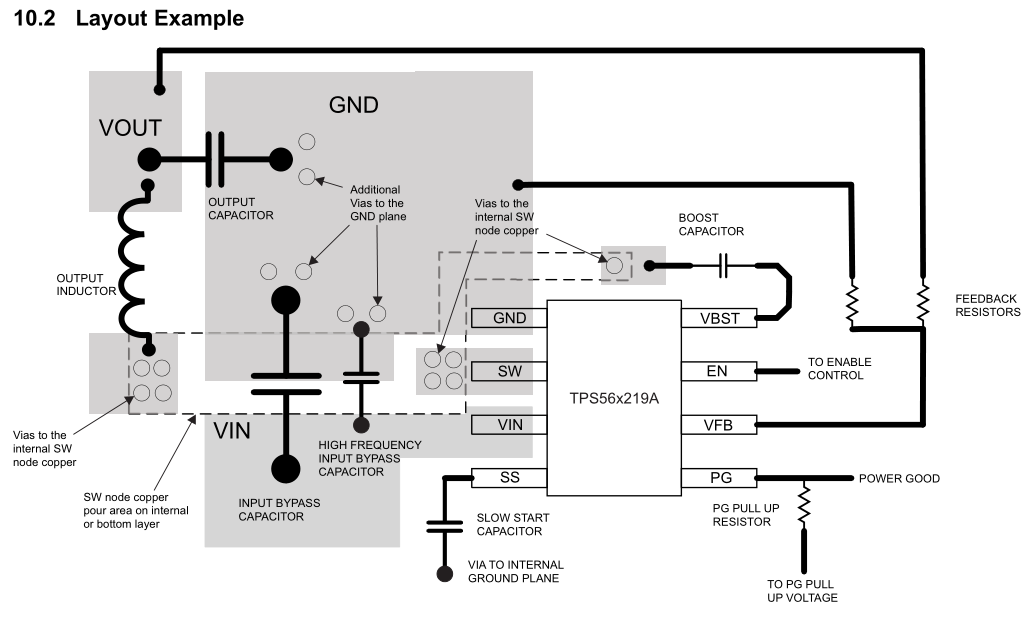
\includegraphics[width=12cm]{resources/pcb_res/tps_logl_example.png}
                \caption{DC/DC elhelyezési mintája}
                \label{fig:tps_logl_example}
            \end{figure}
            
            Az irányelveket követve az elkészült NYÁK-tervet \aref{fig:pcb_3v3} Ábra szemlélteti.
            
            \begin{figure}[h!]
                \centering
                    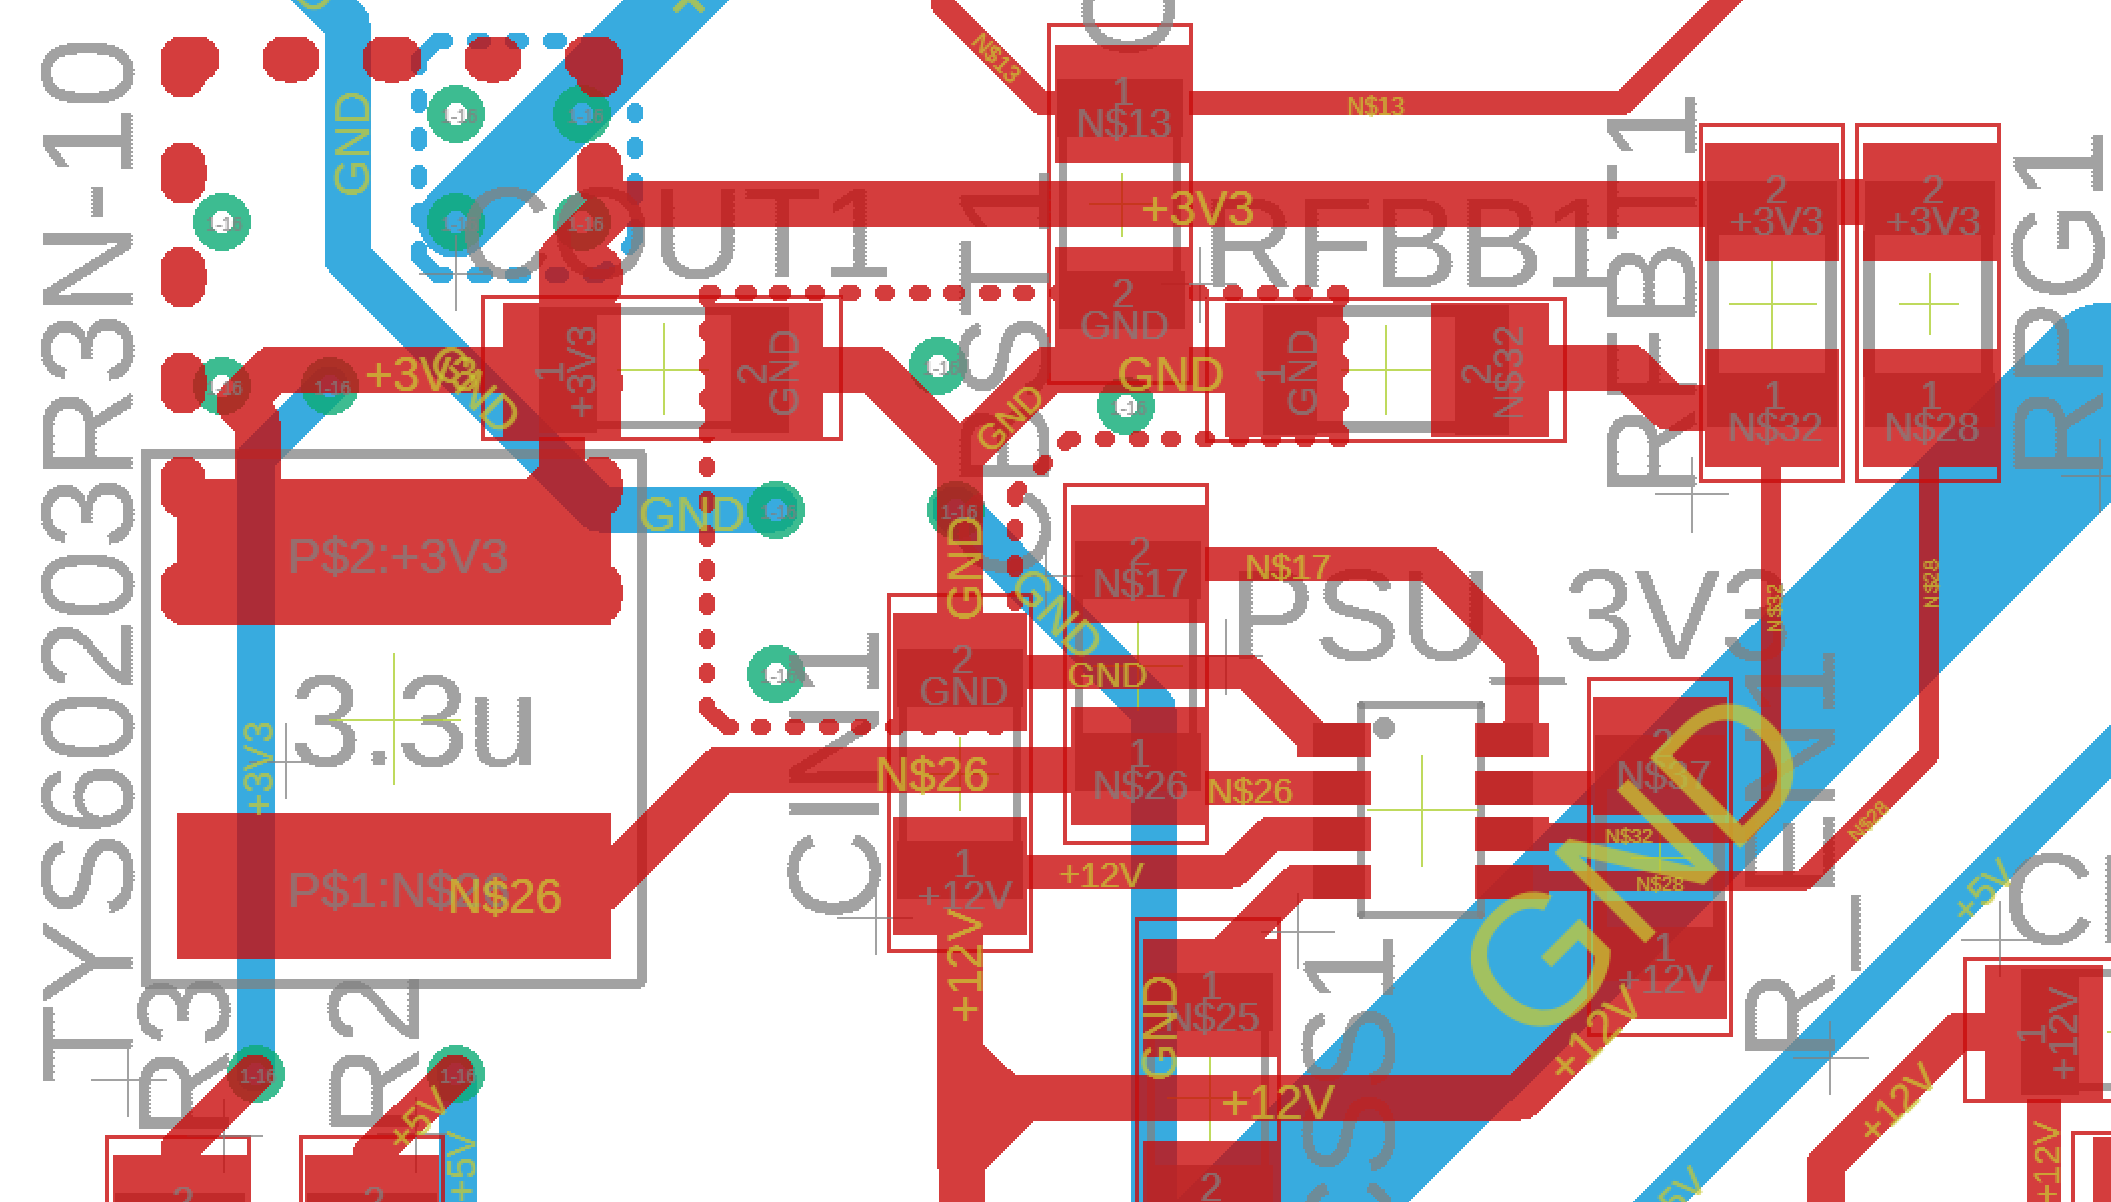
\includegraphics[width=6.5cm]{resources/pcb_res/board_dcdc_3v3.png}
                    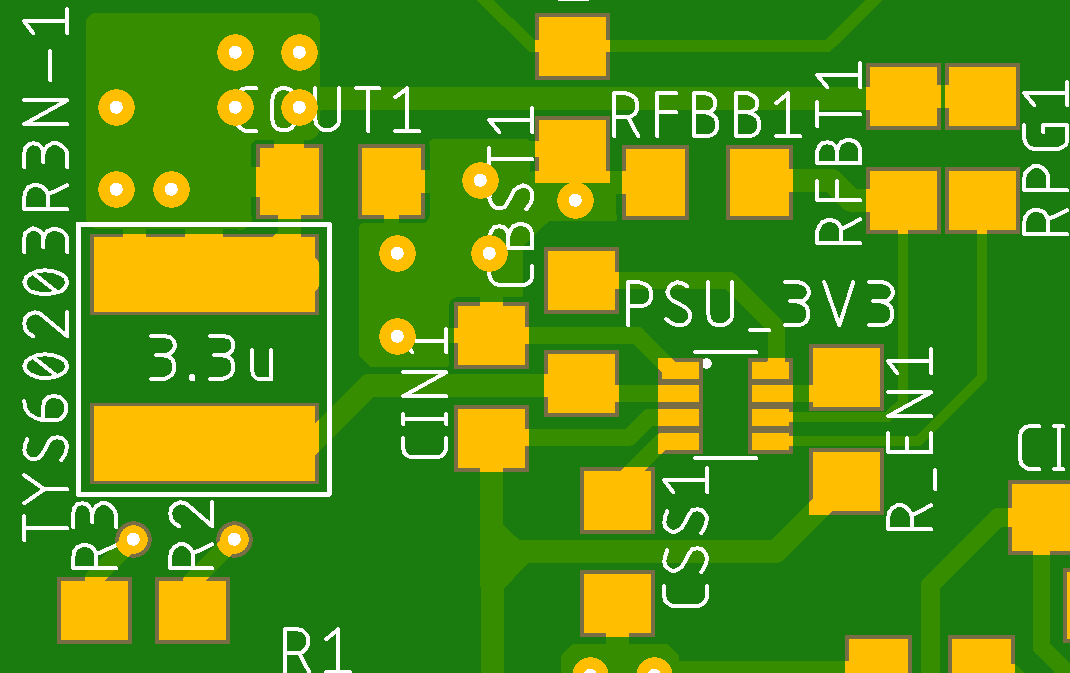
\includegraphics[width=6cm]{resources/pcb_res/pcb_dcdc_3v3.png}
                \caption{3,3V-os DC/DC nyákterve}
                \label{fig:pcb_3v3}
            \end{figure}
            
            Hasonló módon készíttettem el az 5V-os átalakítót is, csak az a NYÁK-on az óra mutató járásával megegyezően 90°-al el lett forgatva.
            
        \subsubsection{Logikai jelszint átalakító tervezése}
            Törekedtem minél több alkatrészemet a TI-től (Texas Instruments) kiválasztani, mert a diákok (érvényes egyetemi e-mail-címmel rendelkezők) számára egy pár ingyenes mintadarabot kínál, amikkel jobb esetben elvégezhető a prototípus fejlesztése. Így esett a választásom a SN74LV1T34 típusú logikai jelszint átalakítóra.
            
            \begin{figure}[h!]
                \begin{floatrow}
                    \ffigbox{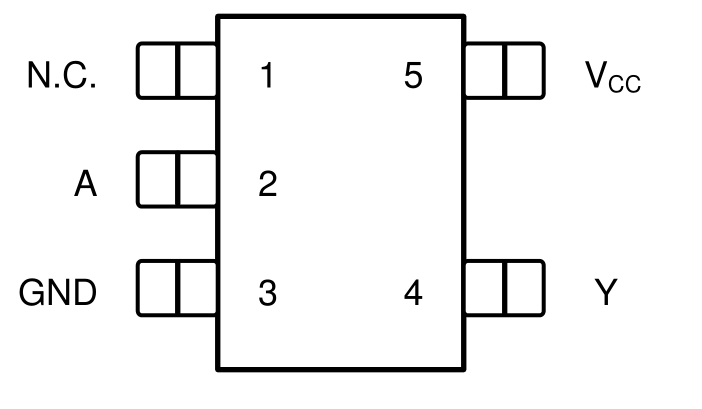
\includegraphics[width=5cm]{resources/pcb_res/SN74LV1T34_pinout.png}}{\caption{SN74LV1T34 logikai jelszint átalakító IC lábkiosztása}\label{fig:SN74LV1T34_pinout}}
                    \ffigbox{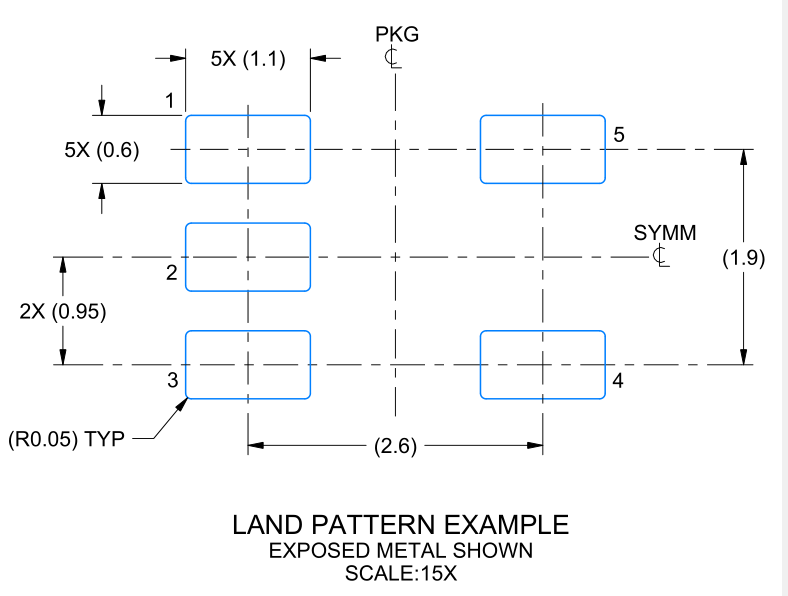
\includegraphics[width=5cm]{resources/pcb_res/SN74LV1T34_land_pattern.png}}{\caption{SN74LV1T34 IC padjeinek elhelyezkedése}\label{fig:SN74LV1T34_land_pattern}}
                \end{floatrow}
            \end{figure}
            
            
            A kis SOT-23-as csomagolású IC (Ábra \ref{fig:SN74LV1T34_pinout}) rendkívül egyszerűvé tette a feladatomat. A 'GND' lábára a földet , az 'A' lábára a bemeneti jelet, az 'Y' lábára a kimenti jelet, a 'V$_{cc}$' lábára pedig a kívánt kimeneti logikai jelszintnek megfelelő 5V tápfeszültséget kellet kötnöm. Az adatlapban leírt forrasztási maszk (Ábra \ref{fig:SN74LV1T34_land_pattern}) alapján elkészíttettem a kis alkatrész Eagle könyvtárát. A 3. fázisú NYÁK-kal már három LED sort szerettem vona vezérelni, ezért a kapcsolási rajzon és a nyákon is három-három darab alkatrész került elhelyezésre.
            
            // képek?? kell/nem?
        
        \subsubsection{STMF103C8T6 mikrokontroller perifériái}
        
        
        
        
        
        
        
//TODO\\
v2 ugyon ugy modulokbol - csak vasalasos technikaval keszitett - mukodik de nem szep, illetve szeretnem emgtanulni a dc/dc tervezest - kepek\\
v3 tervezes legyartas kinaban - kepek\\ 

    \subsection{Forrasztas}
forrasztas - hibajavitas\\
mit csinalnek mashogy legkozelebb\\

doboz tervezese fusionbe - kepek\\
3d nyomtatas - kepek\\
kesz termek - kepek\\

otthoni megvalositas, aramforraskereses, bekotes, zavarszüres ferritgyuruvel, teraszrol kepek\\

Beagyazott szoftver\\
Standard Peripheral Library (spl/stl ?) - a hatterben folyo folyamatok megertese miatt
interrupt, timer, uart, dma kezeles - mit miert
adatszerkezet
kommunikalas az espvel - bekonfiguralasa
ledsorral valo kommunikacio
effektek arduino neopixel librarybol 

\end{document}